\Subsubsection{Naive payment network}
The current form of our payment channel works very well as long as it is between just two parties. A very helpful feature would be to be able to send money to anyone without having a direct channel between you and that person, in other word the transaction jumps between any number of other channels before reaching it's destination. If we naively use the channel we have constructed in the previous section as is to send money over multiple jumps we would run into the following problem:

Imagine there being 3 people: Alice (A), Bob (B) and Cecil (C). Alice and Bob have a channel between each other and Bob and Cecil have a channel between each other. Making the following graph: A - B - C. Alice wants to send money to Cecil but they have no channel between each other. To solve this Alice asks Bob to promise to send x amount of money to Cecil if Alice sends x amount of money to Bob. In the perfect world Bob would be honest and this system of payment networking would work. In the real world however having to trust every node between you and the destination would cause problems with malicious nodes. There is nothing stopping Bob from taking Alice's money and never sending anything to Cecil. 

The channel has to be extended further to allow multi-hop payments and still retain it's breach remedy feature. This is where Hashed Time Locked Contracts come into the picture. 

\Subsubsection{Payment channels with Hashed Time Locked Contracts}
A new mechanism needs to be added to our payment channel to enforce that multi-hop transactions actually make it all the way to their destination while at the same time still retaining the breach remedy mechanism etc... 

This could be done by adding a third output to the commitment transactions. This new output pays to a hashed time locked contract (\textbf{HTLC}). Before when a payment was made over a payment channel the amount was updated for each output representing a user in the channel. With the HTLC-output the amount sent is represented by the the value of the HTLC-output. 

A channel could be thought of as having three states: regular, unsettled, and settled. The regular state is the one described in previous sections, it's a channel with one set of active commits, the commit will not have any HTLC-outputs. A channel where the latest commits has a HTLC-output is considered unsettled. The unsettled state should only exists while there is uncertainty about whether the multi-hop transaction completed or not. You could say that \textbf{the HTLC-output only exists as a contingency}, if both parties cooperate the channel can return to regular state with the channel balances updated accordingly, if the parties cannot agree or for some reason will not cooperate the channel should be close as soon as possible, as to why we will get to that. A channel reaches a settled state when both parties decides to close the channel, it is done by creating one last pair of commitment transactions but without any revocable deliveries. After a channel is settled no further transactions could be exchanged in it safely as the mechanism for preventing old transactions from being broadcast has been removed, instead the commitment transaction should be broadcast and the channel properly closed.

To understand the HTLC-output you first need to understand the general mechanism that is used to ensure that multi-hop transactions work. 

\begin{figure}[H]
	\centering
	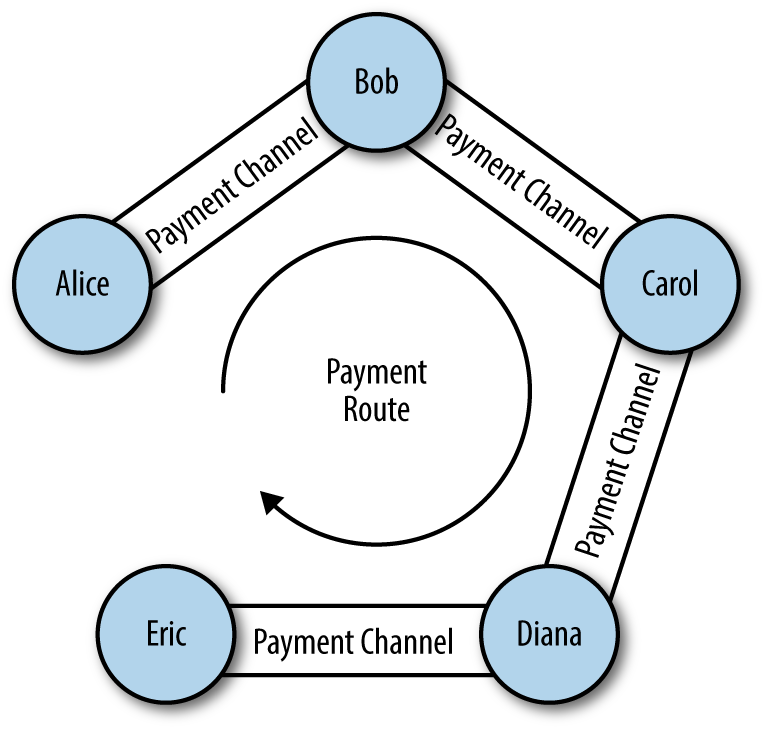
\includegraphics[width=0.55\textwidth]{background/images/pc_route.png}
	\caption{An overview of a network formed by payment channels}
	\label{fig:pc-route}
\end{figure}

The principle used for multi-hop transactions is a lot like the one used for onchain atomic swaps. It relies on revealing a secret pre-image\footnote{See glossary} of a hash within a certain time limit. Using the diagram in figure \ref{fig:pc-route} as example. Alice wants to send money to Eric. But they have no direct channel between each other. To make this work Alice asks Eric for a hash of a secret, let's call this $H = SHA256(R)$. For now Eric holds on to R and only sends H to Alice.

For the money to reach Eric, Alice needs to go via Bob. To do this Alice requests from Bob that they make a new commitment transaction with one HTLC output. The amount in the output should be equal to to whatever amount Alice want to send to Eric. The promise here is that Bob will get this money only if he can prove that he has the pre-image to H. Bob does the same with Carol. This continues until an updated commitment reaches Eric. Eric can then send the pre-image R backwards through the chain until it reaches Alice. 

\begin{figure}[H]
	\centering
	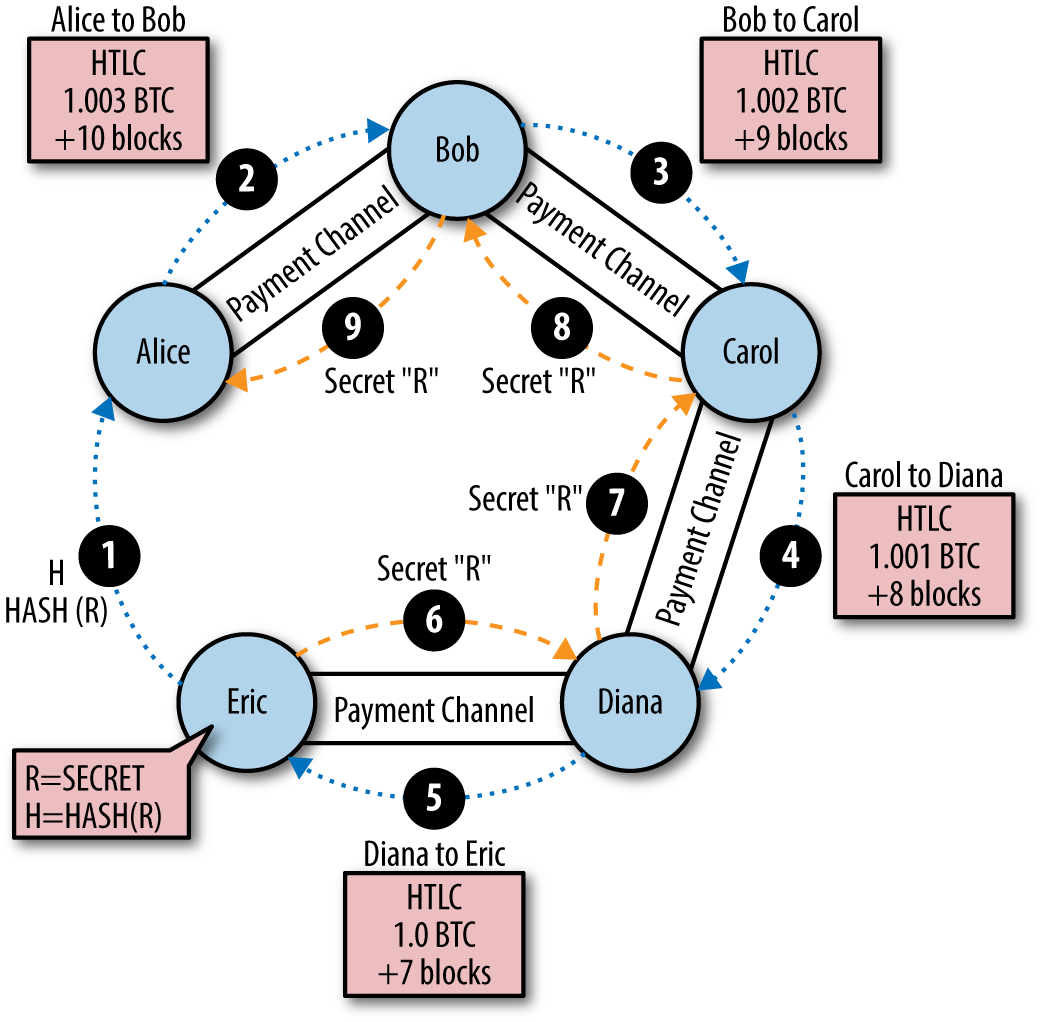
\includegraphics[width=0.75\textwidth]{background/images/pc_route_backwards.png}
	\caption{All the steps taken in the payment network}
	\label{fig:pc-route}
\end{figure}

Earlier it was mentioned that the HTLC output only existed as a contingency, when Bob can prove to Alice that he knows the pre-image R, and can claim the money in the htlc-output by closing the channel, Alice has no reason to not update the channel with correct balances in Bob's favor. Thus the channel returns to a regular state with no htlc-outputs and all previous commits are revoked. This is done for all channels between Alice and Eric. If a party will not co-operate in the chain the channels to that person will have to be closed, this is the only case where the htlc-outputs are actually spent. There is no risk of monetary loss, closing channels is generally something that should be avoided if not absolutely necessary.

\vspace{10mm}
\Subsubsection{HTLC in more detail and second-level HTLCs}
The HTLC script is a bit different depending on what side you are on in the channel, in other words the HTLC in the commitment of the sender is different to the one on the receiver end. 